\section{Text Based Programming Languages}
\label{sec:text_based_programming_languages}
\todo{Watch the smalltalk talk, and maybe add something about it here}\\
Text based programming languages can be split into two categories; one is the text based educational programming languages for novices, and the other are the general purpose programming languages. Event though general purpose programming languages can be used to teach programming to novices, the two categories are distinguished in where the focus of the design has been. This chapter will explore the programming languages in both of these categories.

\subsection{Text Based Educational Programming Languages}
This section will provide a description of some different text based educational programming languages and constructs.
\subsubsection{Turtle Programming}
One of the first programming languages that added constructs for learning programming was LOGO. It did not have the constructs from the start, but after 12 seventh-grade students\footnote{From Muzzy Junior High School in Lexington, Massachusetts.} worked with LOGO for a year (1968-1969), Seymour Papert, one of the developers of LOGO, proposed the Turtle as a programming domain that could be interesting to people at all ages. He proposed it since the demonstration had confirmed that LOGO was a learn able programming language for novices, but he wanted the demonstration extended to lower grades, ultimately preschool children. Constructs for Turtles was then added to LOGO and has since been widely adopted in other programming languages such as SmallTalk and Pascal, and more recently Scratch\cite{turtle_origin}.

A Turtle can be a visual element on a screen or a physical robot. In Scratch, the Turtle can be any sprite chosen by the user. In LOGO the Turtle is controlled by a set of commands which are:
\begin{itemize}
\item FOWARD X, moves the Turtle X number of Turtle steps in a straight line
\item RIGHT X, turns the Turtle X number of degrees in a clockwise direction
\item LEFT X, turns the Turtle X number of degrees in a counter clockwise direction
\item PENDOWN, makes the Turtle draw
\item PENUP, makes the Turtle stop drawing
\end{itemize}
These commands make up the essence of Turtle programming and the functionality is also present in the other languages which has implemented Turtle programming, maybe using different keywords. Some languages has expanded on these commands e.g. in Scratch, one can change the color, size and shade of the pen. The commands can be part of user defined functions. Examples could be functions called \emph{SQUARE} or \emph{TRIANGLE} which would draw a square and a triangle respectively using the commands shown. These functions can be part of other functions, e.g. a function called \emph{HOUSE} would use a mix of the commands for correct positioning and then the \emph{SQUARE} and \emph{TRIANGLE} functions to draw the house itself\cite{turtle_func}.

Turtle programming is not only meant as a tool for learning to program, Seymour Papert states that it is meant as an \emph{Object-to-think-with}. This means that it is supposed to give children a way of relating new topics to something they already know. Alan Kay shows an example of this in a talk, where he uses a car sprite (the turtle in this case) to visualize acceleration. He does this by programming a loop for the car that for each iteration makes a circle showing where the car have been and then moves the car forwards to a new position. In each iteration he also increases the distance that the car moves forwards, meaning that the distance between the circles becomes greater and greater, thus visualizing the car accelerating\cite{alan_turtle_video}.

\subsubsection{Small Basic}
Small Basic is a text based programming language with its whole purpose being teaching novices to program. It is not meant as a language one should keep using, but as a tool for learning programming principles and then ``graduating'' to learn more advanced languages. In the developers internal trials they have had success with teaching programming to kids in the ages of 10 and 16, but it is intended for novices in general, so it is not specifically made for that age group\cite{smallbasic_faq}. It is perhaps one of the last languages with this purpose that is still being updated\footnote{With that being said there was a four year hiatus between version 1.0 and 1.1}. It seems as if the focus of teaching programming to novices has changed to visual programming languages, tools for learning existing languages that is meant to be used professionally or languages that are novice friendly, but still meant to be used professionally.

The Small Basic project consist of three pieces, the language itself, an IDE and libraries. This means that one has to use the bundled IDE to program in Small Basic. According to their FAQ\cite{smallbasic_faq}, the language takes inspiration from an early variant of BASIC but is based on the modern .NET Framework Platform. It is much smaller than Visual Basic, it consists of 14 keywords, and supports a subset of the functionality that Visual Basic .NET supports. It does not have a type system and all variables are global and always initialized as to avoid confusion regarding scopes. It is also imperative and do not use or expose beginners to the concept of object orientation.

To learn programming with Small Basic its website provide a tutorial for getting familiar with the language and the IDE\cite{smallbasic_intro}, and a curriculum, which can be downloaded for offline use, which teaches general programming topics using Small Basic\cite{smallbasic_curriculum}. Through the introduction one will learn that there is to different window types ones program can be run in, either the \emph{TextWindow} which is a regular console, or in the \emph{GraphicsWindow} where graphics can be drawn and so on. So it is possible to create e.g. games in Small Basic. Turtle programming is also supported.

The Small Basic IDE aims to help novices as well. The IDE is made up of different parts which are which can be seen in Figure \ref{fig:small_basic_ide}. The first part is the menu bar in the top, this contains a very limited subset of functionality that we are used to see in regular programming IDEs and a Small Basic specific functionality, the Graduate button. The Graduate button can export the code that has been written in Small Basic to Visual Basic so that the developer can keep programming on their project even if they have ``graduated'' to using Visual Basic instead. The second part is the editor itself, where the code is written. The third part is intelliSense and auto complete. It is works the same as in Visual Studio, it shows what is possible to write with a description of what that functionality does. The fourth part is where the error messages are shown and the fifth part shows the properties of a selected element.

\begin{figure}[H]
\begin{center}
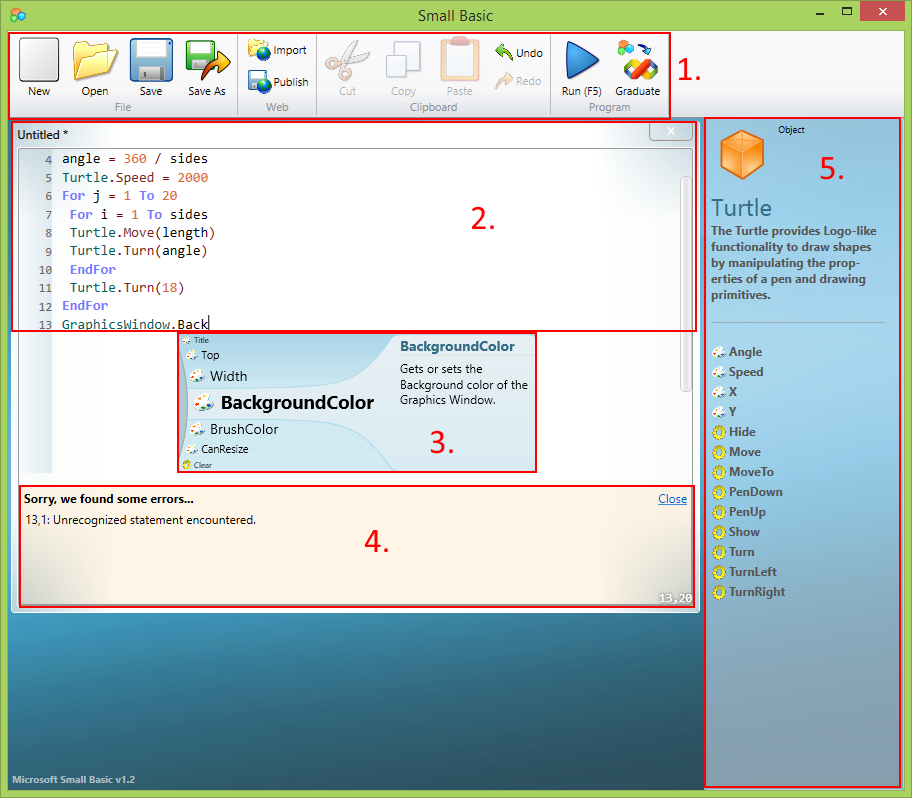
\includegraphics[scale=0.60]{./pics/SmallBasic.png}
\caption{Small Basic IDE}
\label{fig:small_basic_ide}
\end{center}
\end{figure}

\subsection{General Purpose Programming Languages}
This section will provide an overview of some of the general purpose programming languages that has been designed with novices in mind, but still aims to be used as a end-user language. It will also provide an overview of some of the tools used to teach novices to program in languages not specifically designed for novices but as a professional programming language. \todo{We need to discuss terminology further.}

\subsubsection{Programming Languages}
One of the first programming languages designed for novices and to be user friendly is BASIC (Beginner's All-purpose Symbolic Instruction Code). It first appeared in 1964 as a language that would enable students in fields other than science and mathematics to use computers. Since then it became a widely used language and today there are more than 230 different documented dialects of BASIC, among those is Microsoft's Visual Basic.

Another language that was originally designed largely with students in mind was Pascal. It was released in 1970 and aimed to teach students structured programming. It was all that, but some early adopters used it far beyond the original intent. This resulted in a lot of work on Pascal and it evolved, both the language itself but also into different dialects, which ended up being designed more towards end-user use rather than an educational tool. Although this meant that the language and dialects became very popular and widely used. The language itself and the dialect called Delphi/Object Pascal is still used today according to \cite{tiobe}.

A third language that was designed and is still maintained as an easy-to-use general purpose programming language is Quorum. Quorum is what the developers of it call an ``Evidence-based'' programming language. This means that it is updated and changed according to current research on how an easy-to-use programming language should be designed. Some of the team members behind the language hosts an annual workshop called The Experience Programming in Quorum (EPIQ), which is ``an international professional development workshop for educators to learn the foundational skills necessary to teach students computer science using the Quorum programming language''\cite{quorum_epiq}.
\todo{Tools for learning e.g. BlueJ}\\
\todo{Add missing sources!}\\

\todo{Remember to summarize text compared to visual programming.}\\
\todo{transition to visual programming}\\
\todo{Why is it the goal to learn these languages? (Look into Intentional Programming)}\\
\todo{Why can't we stick with the educational ones?}\\
\todo{Why don't we begin with these?}\\
\todo{Good thing about text based, is terminology, one learns to talk about programming, e.g. what is a statement?}

%http://dl.acm.org/citation.cfm?id=1227003
%paper of physical programming

%1: page 218
%2: page 11-15
%3: https://www.youtube.com/watch?v=JDpsXWuedVc
%4: http://smallbasic.com/faq.aspx
%5: http://download.microsoft.com/download/9/0/6/90616372-C4BF-4628-BC82-BD709635220D/Introducing%20Small%20Basic.pdf
%6: http://social.technet.microsoft.com/wiki/contents/articles/16982.small-basic-curriculum-online.aspx
%7: http://www.tiobe.com/index.php/content/paperinfo/tpci/index.html
%8: http://quorumlanguage.com/epiq.php